\documentclass[a4paper,12pt]{article} 

%Добавляет возможность искать и копировать текст
\usepackage{cmap}

%Убирает пробел между названием таблицы/рисунка и самой таблицей/рисунком
\usepackage{caption}
\captionsetup[table]{skip= -0 cm}
\captionsetup[figure]{skip= -0 cm}

%Выравнивание названия таблиц по левому краю
%\usepackage[nooneline]{caption} 
%Размеры отступов 
\usepackage[left=20mm, top=20mm, right=20mm, bottom=20mm, footskip=10mm]{geometry}

%Рисунки
\usepackage{graphicx}
\usepackage{wrapfig} %обтекание элементов
\graphicspath{{graphs}{figures}}  % папки с картинками

%Русский язык в формулах
%\usepackage{mathtext}

%  Русский язык
\usepackage[T2A]{fontenc}			
\usepackage[utf8]{inputenc}			
\usepackage[english,russian]{babel}	

%Готические буквы
\usepackage{amssymb}

% Математика
\usepackage{amsmath,amsfonts,amssymb,amsthm,mathtools} 
\usepackage{wasysym}

%Цветные подписи в таблице
\usepackage[table,xcdraw]{xcolor}

\usepackage{fancyhdr} % Колонтитулы
 	\pagestyle{fancy}
 	\renewcommand{\headrulewidth}{0.3mm}  % Толщина линейки, отчеркивающей верхний колонтитул
 	%\lfoot{Нижний левый}
 	%\rfoot{Нижний правый}
 	\rhead{Кафедра вакуумной электроники}
 	%\chead{Верхний в центре}
 	\lhead{Конвективная диффузия}
 	% \cfoot{Нижний в центре} % По умолчанию здесь номер страницы
 	
\begin{document} 

%Титульник 
\begin{titlepage}
	\begin{center}
		\large 	МИНИСТЕРСТВО ОБРАЗОВАНИЯ И НАУКИ РОССИЙСКОЙ ФЕДЕРАЦИИ\\
				МОСКОВСКИЙ ФИЗИКО-ТЕХНИЧЕСКИЙ ИНСТИТУТ \\
				(НАЦИОНАЛЬНЫЙ ИССЛЕДОВАТЕЛЬСКИЙ ИНСТИТУТ)\\ 
				ФИЗТЕХ-ШКОЛА ЭЛЕКТРОНИКИ, ФОТОНИКИ \\
				И МОЛЕКУЛЯРНОЙ ФИЗИКИ \\
		
		
		\vspace{4.0 cm}
		\LARGE{Кафедра вакуумной электроники \\ 
		Отчет по лабораторной работе} \\ 
		\LARGE \textbf{Конвективная диффузия в молекулярно-электронных преобразователях} \\
	\end{center}
	\vspace{3 cm} \large

	%Надо подумать как это нормально написать	
	\begin{flushleft}
		Работу выполнили \hspace{5.5cm}  \underline{\hspace{3cm}} А.И.Белостоцкий \\	
		\hspace{9.8cm}  \underline{\hspace{3cm}} Д.Е.Вовк \\
		\hspace{9.8cm}  \underline{\hspace{3cm}} А.Кадыров \\
		\hspace{9.8cm}  \underline{\hspace{3cm}} Г.Мусатов \\
		\vspace{2cm}
		Работу принял, оценка \hspace{4.3cm} \underline{\hspace{3cm}}
	\end{flushleft}
	
	
	\vfill

	\begin{center}
	Долгопрудный, 2022 г.
	\end{center}
\end{titlepage}                                                                      

\tableofcontents

\newpage

\section{Цель работы}
Исследование процессов протекания тока в молекулярно-оптическом преобразователе в стационарных и нестационарных условиях

\section{Экспериментальная установка}

\begin{figure}[h]
	\begin{center}
		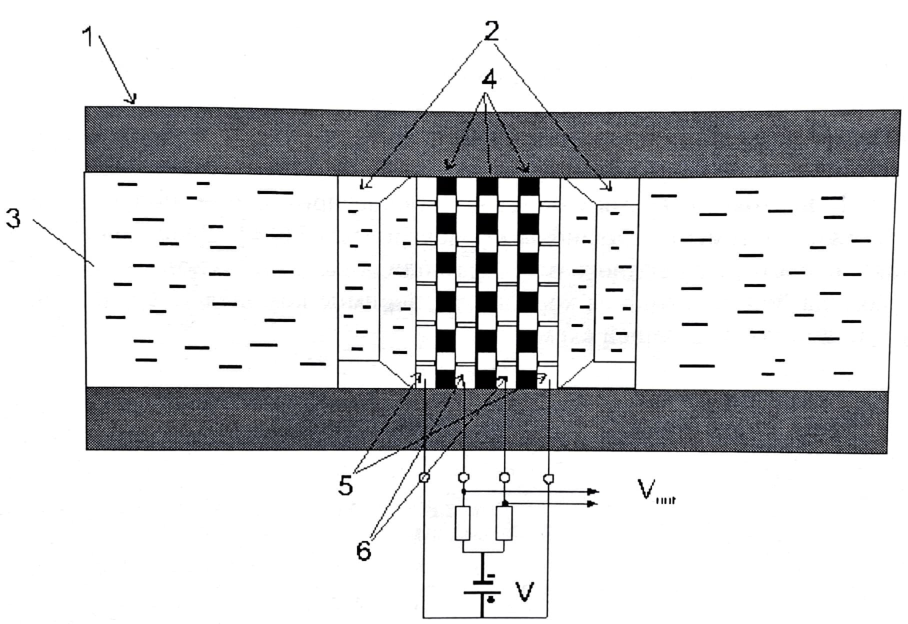
\includegraphics[scale=1]{fig1}
		\caption{Молекулярно-электронный преобразователь}
		\label{MEP}
	\end{center}
\end{figure}


Принципиальная схема молекулярно-электронного преобразователя (МЭП) показана на рис. \ref{MEP}. Он представляет собой электродный узел -- 2, помещённый в диэлектрическую трубку -- 1, заполненную раствором электролита -- 3. Внутри электродного узла установлены четыре плоских сетчатых электрода (аноды -- 5 и катоды --6) , разделённые пористыми перегородками -- 4.

Работа МЭП основана на том, что прохождение тока через электрохимическую ячейку в значительной степени определяется гидродинамическим движением раствора, вызванным действием внешних возмущений. В МЭП скорость химической реакции на электродах ЭЯ значительно больше скорости доставки к ним реагирующих веществ. В этом случае при протекании реакции в ЭЯ появляется градиент концентрации реагирующих веществ и перенос заряда в неподвижном электролите осуществляется с помощью диффузии ионов от одного электрода к другому. Если жидкость приходит в движение, то наряду с диффузией возникает конвективный перенос ионов, что резко изменяет скорость доставки реагирующих веществ к электродам и соответственно ток, идущий через ЭЯ.

В МЭП могут быть использованы различные окислительно-восстановительные реакции, например: йод-йодид, ферро-Феррицианид и др. При этом чаще всего электроды ЭЯ изготавливаются из металла, который не участвует в обмене катионами, а осуществляет только электронный обмен.

\section{Теоретические сведения}

\subsection{Математическое описание переноса тока в ЭЯ}

Математическая формулировка задачи для расчета тока, текущего через электрохимическую ячейку, сводится к решению уравнений гидродинамики и диффузии:

\begin{gather}
\frac{\partial \mathbf{v}}{\partial t} + (\mathbf{v}, \nabla)\mathbf{v} = -\frac{\nabla \rho}{\rho} + \mathbf{j} \nabla \mathbf{v},  \\
%
\operatorname{div} \mathbf{v} = 0, \\
%
\frac{\partial n}{\partial t} = D \Delta n + (\eta, \nabla)n,
\end{gather}

где $\mathbf{v}$ -- скорость электролита, p -- давление, $\rho$ -- плотность, $\rho$ -- вязкость жидкости, n -- концентрация носителей тока (ионов трийодида), D -- коэффициент их диффузии, j -- плотность потока. В системе с плоскими электродами эти уравнения фактически являются одномерными.

В качестве граничных условий к уравнениями (1) -- (3) используются следующие соотношения:

\begin{itemize}
\item Отсутствие потока активных ионов через диэлектрические поверхности.
\item Уравнения, определяющие скорости электрохимических реакций в зависимости от
концентрации ионов и скачка потенциала на границе электрод/электролит.
\end{itemize}

Кроме того, дополнительно накладывается интегральное соотношение, выражающее закон сохранения количества активных ионов

\begin{equation}
	\iiint n(x, y, z, t) dV = V n_0,
\end{equation}

где V -- объем  электролита, $n_0$ -- равновесная концентрация. 

Следует отметить, что система уравнение (1) -- (3) является приближенной и не учитывает наличие в МЭЯ электрического поля и объемного заряда.

\subsection{Стационарный случай}

Как известно, величина а диффузионного тока, текущего через электрод, определяется выражением:

\begin{equation}
	I_D = - e S D \nabla n,
\end{equation}

где S -- площадь электродов.

Используя соотношение (5)б получим вольт-амперную характеристику молекулярно-электронной ячейки с неподвижным электролитом. Для простоты будем считать, что линейные размеры электродов много больше расстояния d между ними. В стационарном случае уравнение диффузии (3) имеет вид

\begin{equation}
	\Delta n = 0
\end{equation}

\begin{figure}[h]
	\begin{center}
		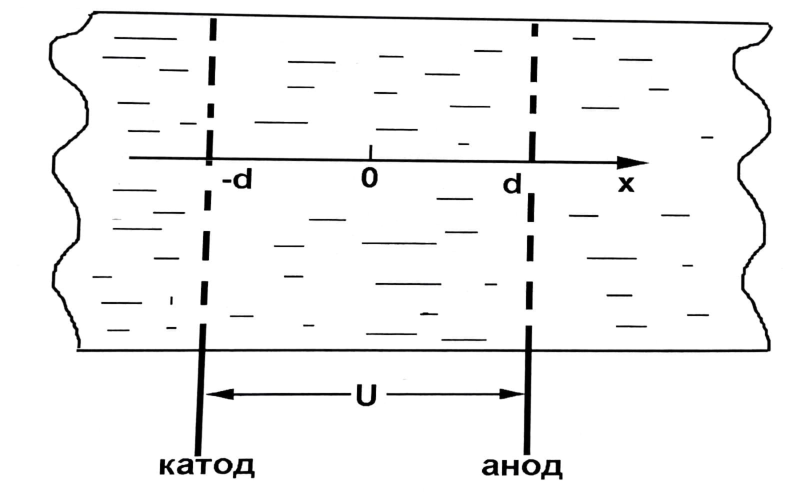
\includegraphics[scale=0.8]{fig2}
		\caption{МЭЯ с плоскими проницаемыми электродами}
		\label{MEYA}
	\end{center}
\end{figure}

\newpage

Один из способов представления граничных условий:

\begin{gather}
n_a = n(d), n_k = n(-d), \\
%
\int\limits_{-d}^{d} n(x,t) dx = 2 d n_0	, \\
%
n_a = n_k exp\left(\frac{eU}{k_{Б} T}\right).
\end{gather}

Решение уравнения (6) имеет вид

\begin{equation}
n(x) = Ax + B
\end{equation}

константы интегрирования определяются из условий (7) -- (9) и записываются в виде:

\begin{gather}
A = \frac{n_0}{d} \tanh\left(\frac{eU}{2 k_{Б} T}\right), \\
%
B = n_0.
\end{gather}

Тогда ток, текущий через катод или анод:

\begin{equation}
I_D  = - \frac{e S D n_0}{d} \tanh\left(\frac{eU}{2 k_{Б} T}\right)
\end{equation}

При $U \gg \frac{k_{Б} T}{e}$:

\begin{equation}
I_0 = - \frac{e S D n_0}{d}
\end{equation}

\newpage

\begin{figure}[h]
	\begin{center}
		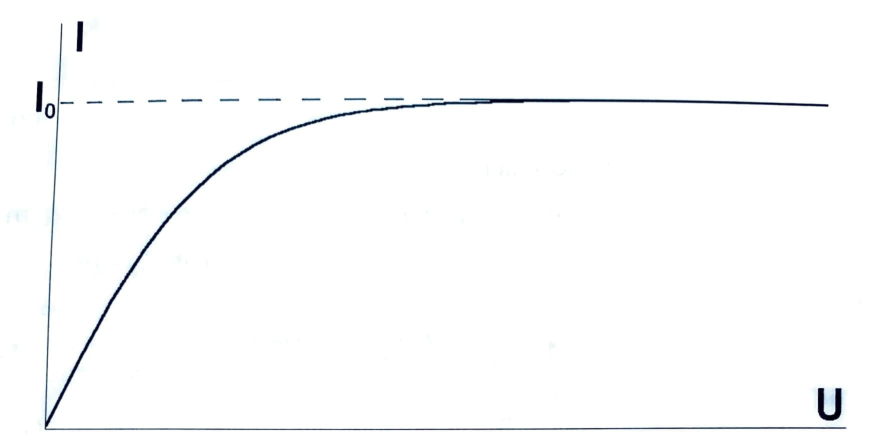
\includegraphics[scale=0.8]{fig3}
		\caption{ВАХ МЭЯ с неподвижном электролитом}
		\label{VAH}
	\end{center}
\end{figure}

\subsection{Конвективная диффузия}

Если жидкость в ЭЯ приходит в движение под действием каких-либо внешних сил, то, наряду с диффузионным, появляется также конвективный ток, обусловленный увлечением ионов движущейся жидкостью. В линейном приближении конвективный ток пропорционален скорости движущейся жидкости V и определяется соотношением:

\begin{equation}
I_k = e S n V
\end{equation}

Для расчёта передаточной функции ЭЯ с плоскими сетчатыми электродами будем использовать модель Лакрама, которая предполагает, что электролит может свободно протекать через электродную систему. В то же время в плоскости анода и катода поддерживаются постоянные концентрации электролита: на аноде $n = 2 n_0$, на катоде $n = 2 n_0 \exp \left(- \frac{eU}{k T} \right)$. Скорость движения раствора под действием внешнего механического
возмущения не зависит от координат и равна $V = V_0 e^{i \omega t}$.

Найдем изменение тока через молекулярно-электронный преобразователь, вызванное протеканием электролита. В случае малых изменений механических величин можно ограничиться линейным приближением. В этом приближении ведем для удобства новую переменную c(x,t), которая определяется из выражения

\begin{equation}
n = n_0\left( 1 - \frac{x}{d}\tanh\left(\frac{eU}{2 k_{Б} T}\right) \right) + c(x, t)
\end{equation}

Будем считать, что c(x,t) малая добавка к концентрации пропорциональна скорости течения жидкости. В этом случае уравнение конвективной диффузии (3) перепишем в следующем виде: 

\begin{equation}
\frac{\partial c}{\partial t} - D \frac{\partial^{2} c}{\partial x^{2}}=V_{0} e^{i \omega t} \frac{n_{0}}{d} \tanh \left(\frac{e U}{2 k T}\right)
\end{equation}

Учитывая граничные условия (9) -- (11) выражение для c(x,t): 

\begin{equation}
c(x, t)=i \frac{V_{0} n_{0}}{d \omega} \tanh \left(\frac{e U}{2 k T}\right) e^{i \omega t}\left(\frac{\operatorname{ch}\left((1+i) \sqrt{\frac{\omega}{2 D}} x\right)}{\operatorname{ch}\left((1+i) \sqrt{\frac{\omega}{2 D}} d\right)}-1\right)
\end{equation}

\newpage

Подставляя (18) в (5), получим выражение для полного тока, текущего через систему:

\begin{equation}
I=-\frac{e S D n_{0}}{d} \tanh \left(\frac{e U}{2 k T}\right)\left[1-e^{i \omega t}(1-i) \sqrt{\frac{1}{2 \omega D}} V_{0} \tanh \left((1+i) \sqrt{\frac{\omega}{2 D}} d\right)\right]
\end{equation}

\begin{figure}[h]
	\begin{center}
		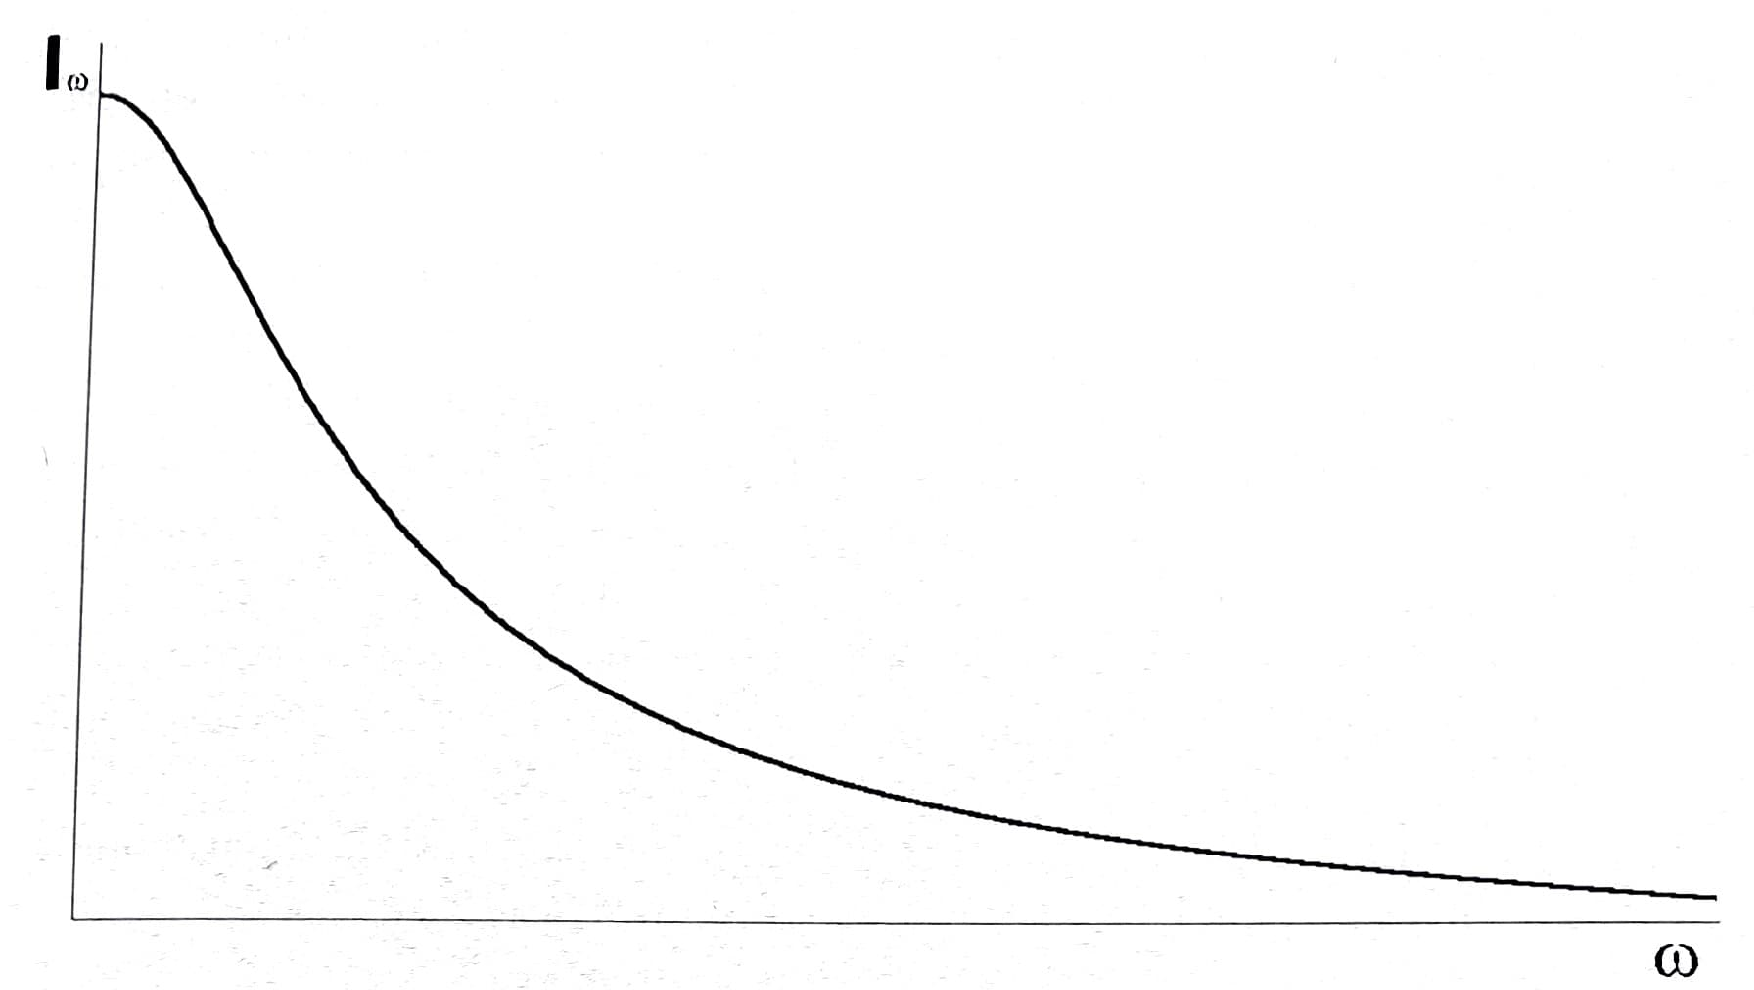
\includegraphics[scale=0.5]{fig4}
		\caption{Зависимость модуля выходного тока МЭП от частоты в условиях конвективной диффузии}
		\label{Module}
	\end{center}
\end{figure}

\section{Ход работы}

\begin{figure}[h!]
	\begin{center}
		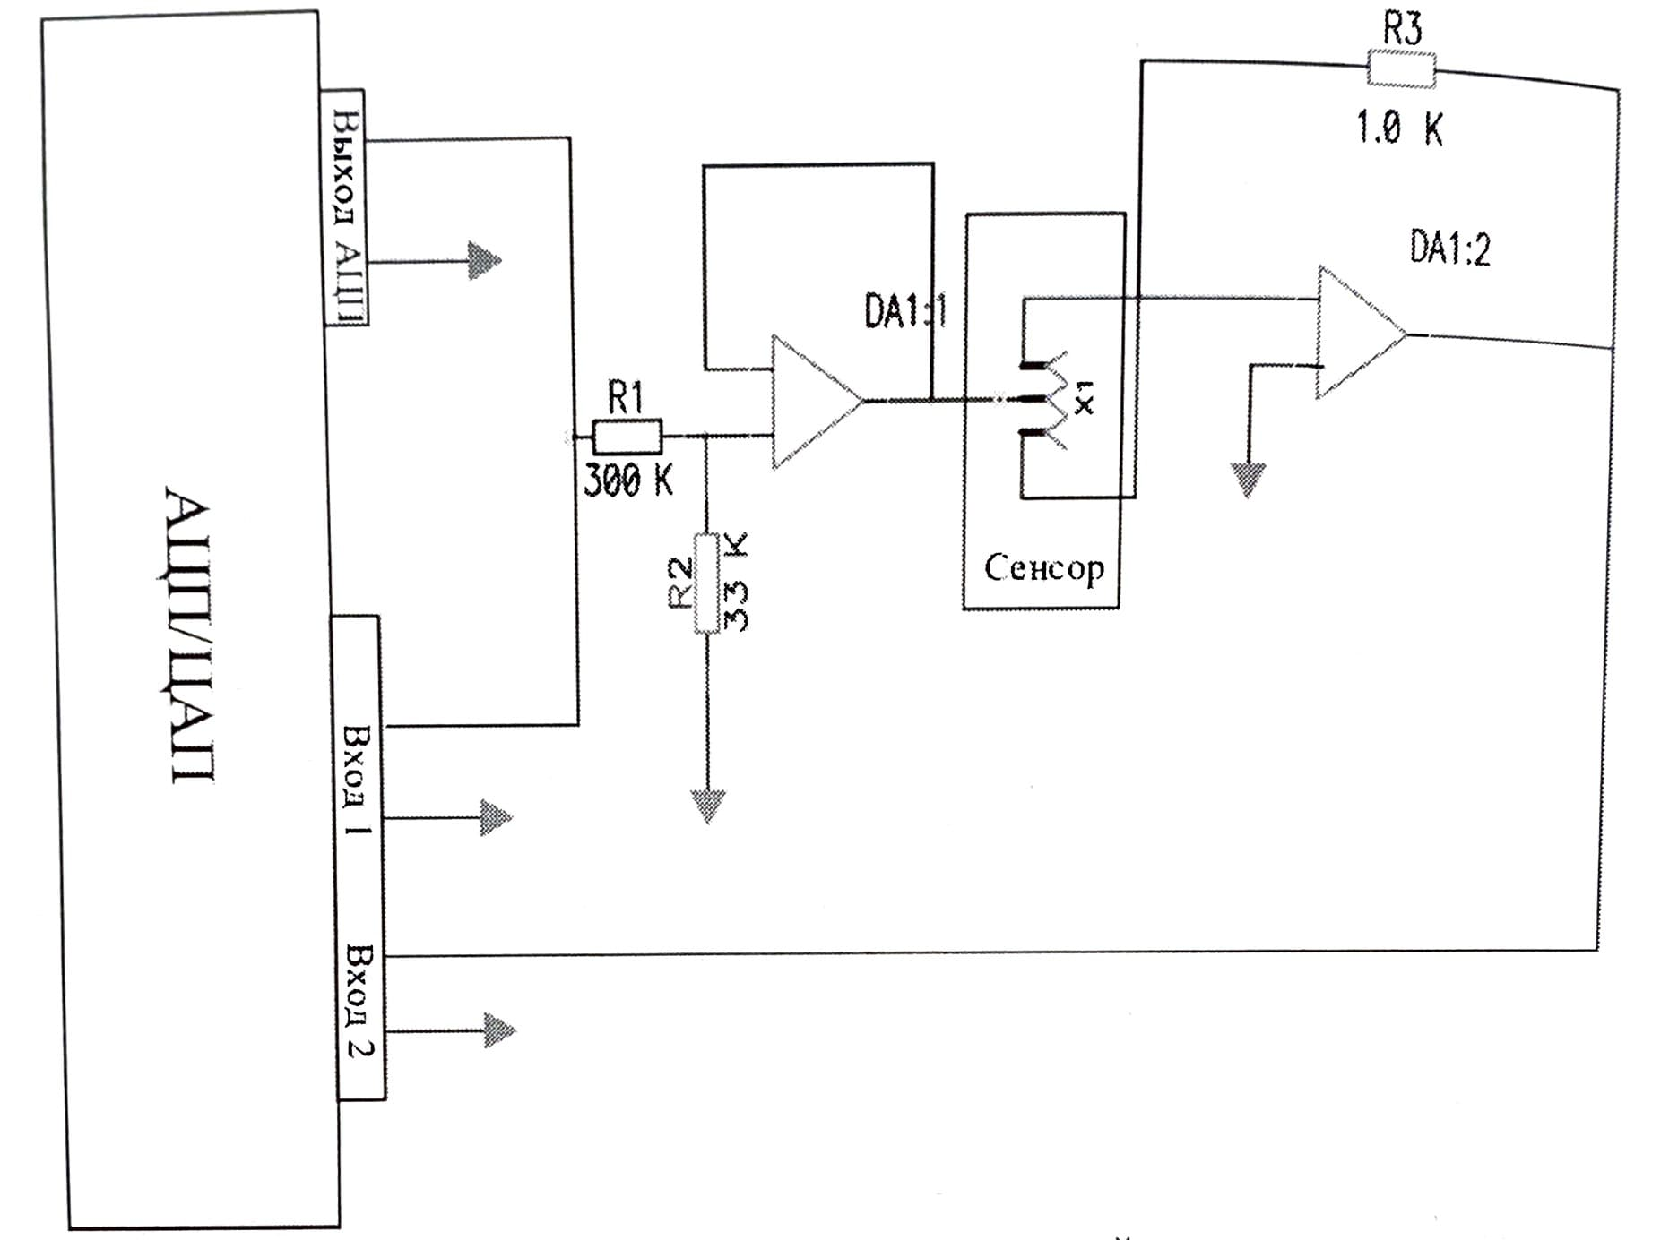
\includegraphics[scale=0.4]{fig5}
		\caption{Принципиальная схема экспериментальной установки для измерения стационарной ВАХ}
		\label{scheme}
	\end{center}
\end{figure}

\newpage

Для стационарного случая проводится измерение BAX, т.е. зависимости выходного тока ЭЯ в условиях стационарной диффузии от приложенной к электродам разности потенциалов. Принципиальная схема экспериментальной установки приведена на рис. 5.

На генераторе сигналов (используется ЦАП) выставляется амплитуда переменного сигнала 0 мВ при произвольной частоте работы генератора. Частота в ходе измерения не изменяется. Величина смещения последовательно изменяется от 0 до 150 мВ в соответствии со значениями приведенными в верхней строчке таблицы 1 Сигнал подается на обе пары электродов молекулярно-электронного преобразователя и контролируется АЦП (канал 2). Суммарный ток с катодов подается на вход операционного усилителя, в обратной связи
которого стоит сопротивление $R_3$ = 1 кОм 

Выходное напряжение операционного усилителя измеряется АЦП (канал 1). Как видно из принципиальной схемы, выходной ток МЭЯ определяется соотношением:

\[
I_D = \frac{U_2}{R}
\]

После изменения смещения необходимо дождаться стабилизации выходного тока (канал 2). После этого ЦАП останавливается (кнопка "stop"), выставляется новое значение смещения и ЦАП запускается повторно. Полученные данные загружаются в Dadisp. В одно из окон загружается входной сигнал (канал 2), в другое -- выходной сигнал (канал 1). Для анализа используются участки записи, соответствующие стабилизации выходного тока. Один отсчет АЦП соответствует 1 мкВ. Данные представлены в Таблице 1.

\begin{table}[h]
\begin{center}
\caption{Измерение ВАХ}
\begin{tabular}{|cl|cl|c|c|c|c|c|c|c|c|}
\hline
\multicolumn{2}{|c|}{$U_{вх}$, mV}   & \multicolumn{2}{c|}{2}       & 10      & 15      & 20      & 30      & 40      & 50     & 100     & 150     \\ \hline
\multicolumn{2}{|c|}{$U_{цап}$, mkV} & \multicolumn{2}{c|}{2000}    & 10000   & 15000   & 20000   & 30000   & 40000   & 50000  & 100000  & 150000  \\ \hline
\multicolumn{2}{|c|}{$U_{ацп}$, mkV} & \multicolumn{2}{c|}{141766}  & 179637  & 176282  & 178338  & 177799  & 175218  & 176260 & 178246  & 174868  \\ \hline
\multicolumn{2}{|c|}{I, mkA}      & \multicolumn{2}{c|}{141,766} & 179,637 & 176,282 & 178,338 & 177,799 & 175,218 & 176,26 & 178,246 & 174,868 \\ \hline
\end{tabular}
\end{center}
\end{table}

По данным Таблицы 1 построим зависимость I(U)

\begin{figure}[h!]
	\begin{center}
		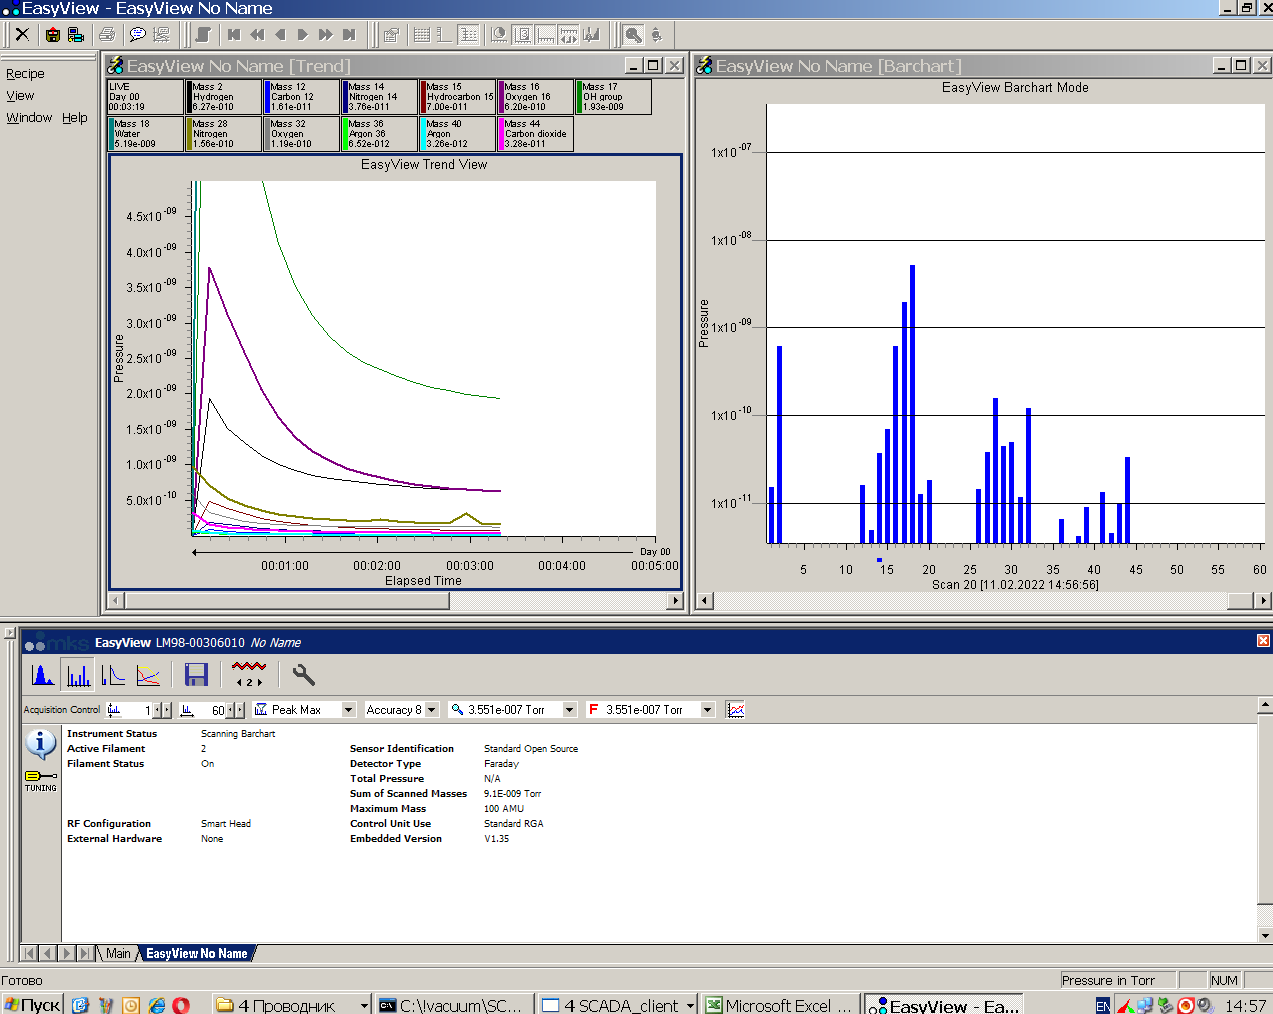
\includegraphics[scale=0.4]{graph1}
		\caption{ВАХ молекулярно-электронной ячейки с неподвижным электролитом}
	\end{center}
\end{figure}

Зная значение $I_0$(из графика), значение коэффициента диффузии носителей тока -- D -- и их равновесную концентрацию -- $n_0$ -- по формуле (14) можно оценить эффективную площадь электродов:

\[
S = \frac{I_0 d}{e D n_0}
\]

Измерения нестационарного (сигнального) тока проводятся с использованием установки, схема которой показана на рис. 7. Экспериментальный образец датчика оснащен электродинамическим механизмом для возбуждения механического воздействия. Принцип возбуждения основана том что сила, действующая на магнит, взаимодействующий с катушкой, пропорциональна величине этого тока. В свою очередь, данная сила эквивалентна силе инерции, т.е. ускорению. Таким образом, изучая зависимость выходного сигнала от тока в катушке возбуждения, можно получить АЧХ сенсора по ускорению с точностью до постоянного множителя (см. рис. )


\begin{figure}[h!]
	\begin{center}
		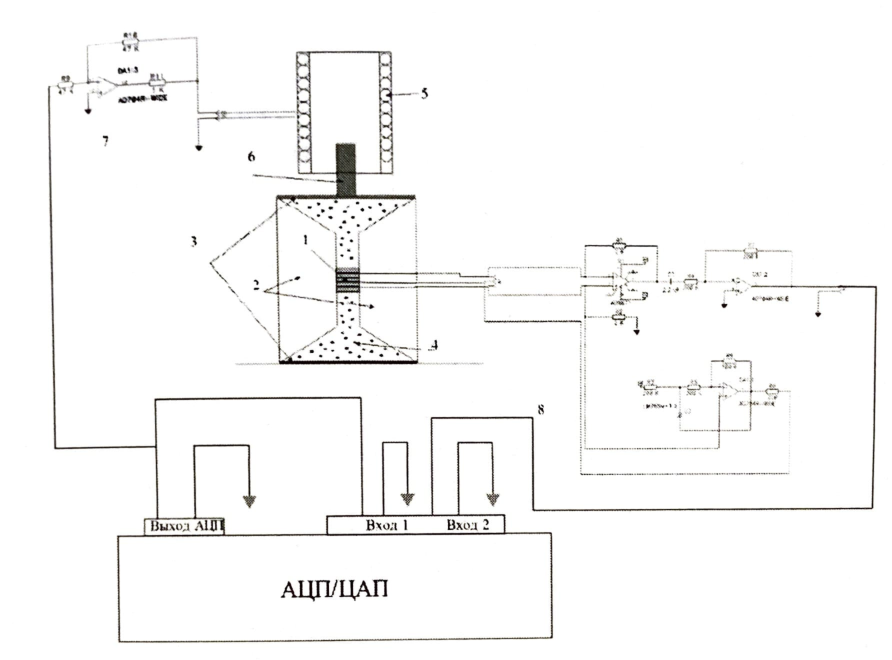
\includegraphics[scale=0.8]{fig6}
		\caption{Принципиальная схема исследования конвективной диффузии в электрохимической ячейке МЭП}
	\end{center}
\end{figure}

Сигнал возбуждения создается с помощью ЦАП, для чего выход ЦАП через электронику возбуждения сигналов 7 подключается к катушке. Величина сигнала возбуждения контролируется АЦП (канал 1). Выходные сигналы электроники для съема сигнала 2 также подключаются к входам АЦП (вход 2). В ходе выполнения измерений постоянное смещение на выходе ЦАП задается равным нулю, амплитуда выходного сигнала постоянной (рекомендуемое значение 25 мВ) а частота последовательно изменяется в диапазоне 0.1 -- 20 Гц. Результаты измерений представлены в Таблице 2.

\newpage

\begin{table}[h!]
\begin{center}
\caption{измерение АЧХ}
\begin{tabular}{|c|c|c|c|c|c|c|c|c|}
\hline
$\nu$, Hz        & 0,1    & 0,2    & 0,5    & 1      & 2      & 5      & 10     & 20     \\ \hline
$\Delta U_{in}, mk$     & 200000 & 200001 & 200002 & 200003 & 200004 & 200005 & 200006 & 200007 \\ \hline
$\Delta U_{out} mk$  & 94261  & 94907  & 93938  & 84415  & 72633  & 54717  & 33250  & 20176  \\ \hline
$\frac{\Delta U_{out}}{\Delta U_{in}}$ & 0,471  & 0,475  & 0,470  & 0,422  & 0,363  & 0,274  & 0,166  & 0,101  \\ \hline
$\ln(\nu)$      & -2,303 & -1,609 & -0,693 & 0,000  & 0,693  & 1,609  & 2,303  & 2,996  \\ \hline
$\ln(\frac{\Delta U_{out}}{\Delta U_{in}})$  & -0,752 & -0,745 & -0,756 & -0,863 & -1,013 & -1,296 & -1,794 & -2,294 \\ \hline
\end{tabular}
\end{center}
\end{table}

По данным Таблицы 2 построим зависимость $ln(\frac{U_{out}}{U_{in}}) (ln(\nu))$

\begin{figure}[h!]
	\begin{center}
		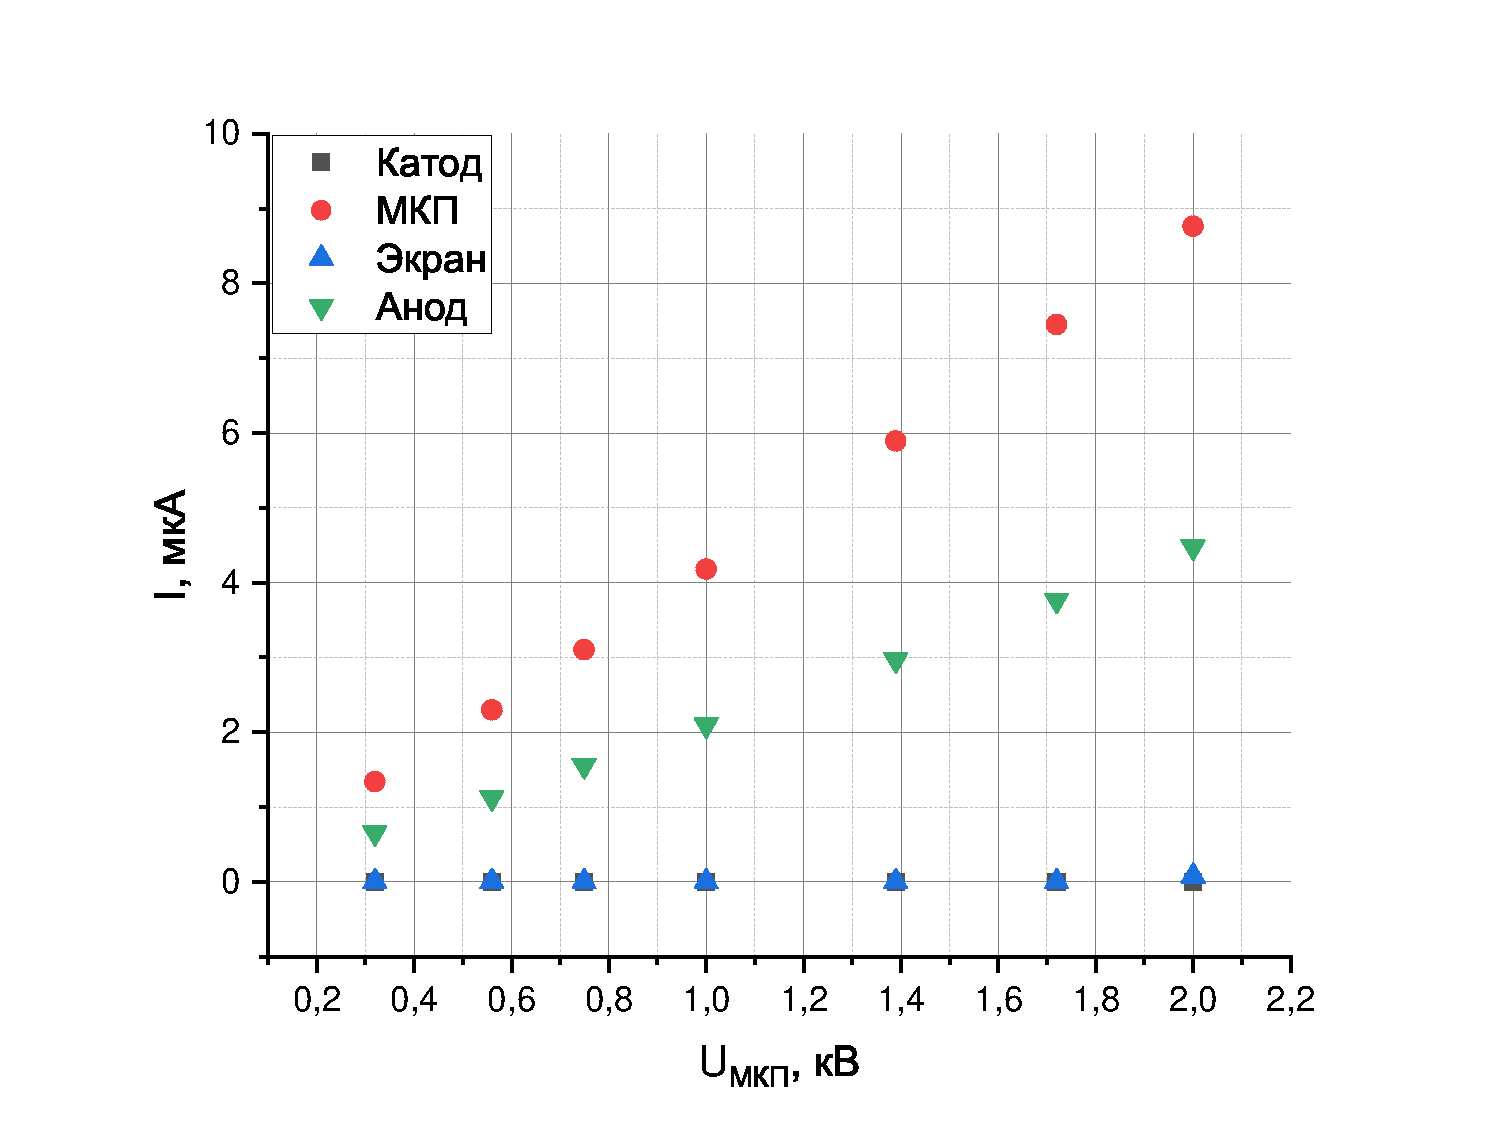
\includegraphics[scale=0.6]{graph2}
		\caption{АЧХ в двойном логарифмическом масштабе}
	\end{center}
\end{figure}

\section{Выводы}
1.В результате работы, мы исследовали процессы протекания тока в молекулярно-электронном преобразователе в стационарных и нестационарных условиях.























\end{document}